\chapter{Formal Analysis Using Alloy}
In this section will be provided a formal model of the problem achieved using Alloy. \\
The model represent only the most important part of the problem, few things have been simplified leaving the more relevant constraints.
For the sake of readability the generated world is splitted in three sub-world which will be explained below.

\section{Alloy Model}
\lstinputlisting[language=alloy]{alloy/model.als}

\subsection{First World}
In the first world (Figure \ref{fig:world1}) the focus is on the \textbf{store} and the \textbf{ticket feature}. In the store there all its informations,
the manager user and employee user. The store has also a ticket queue which contains only tickets that has the status \textit{VALID}. 
In case of a ticket \textit{EXPIRED} or \textit{USED}, the ticket is removed from the queue.
\subsection{Second World}
In the second world (Figure \ref{fig:world2}) the focus is on the \textbf{booking feature}. Store has timeslots which were hidden in the previous world. They represent a slice of time that can be booked.
Every booking must book at least one timeslot.
\subsection{Third World}
In the third world (Figure \ref{fig:world3}) the focus is on a \textbf{multiple store} implementation. Every store has its informations and its manager and employee users. It is notable that the CLup admin
is \textit{super partes} and has no relation with the number of store.

\begin{figure}[H]
	\centering
	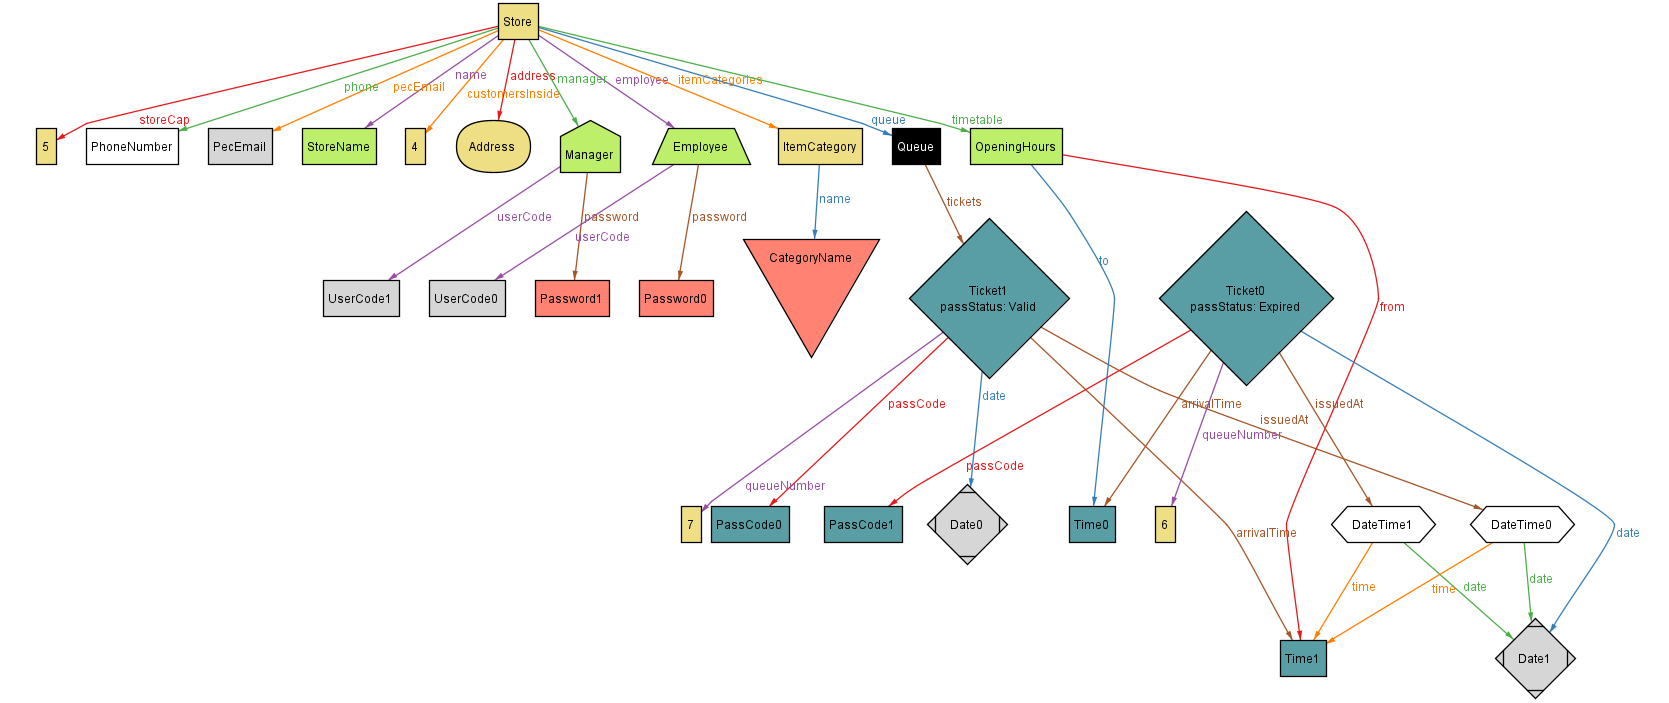
\includegraphics[angle=90,origin=c,height=\textwidth]{world1}
	\caption{First World.}
	\label{fig:world1}
\end{figure}
\begin{figure}[H]
	\centering
	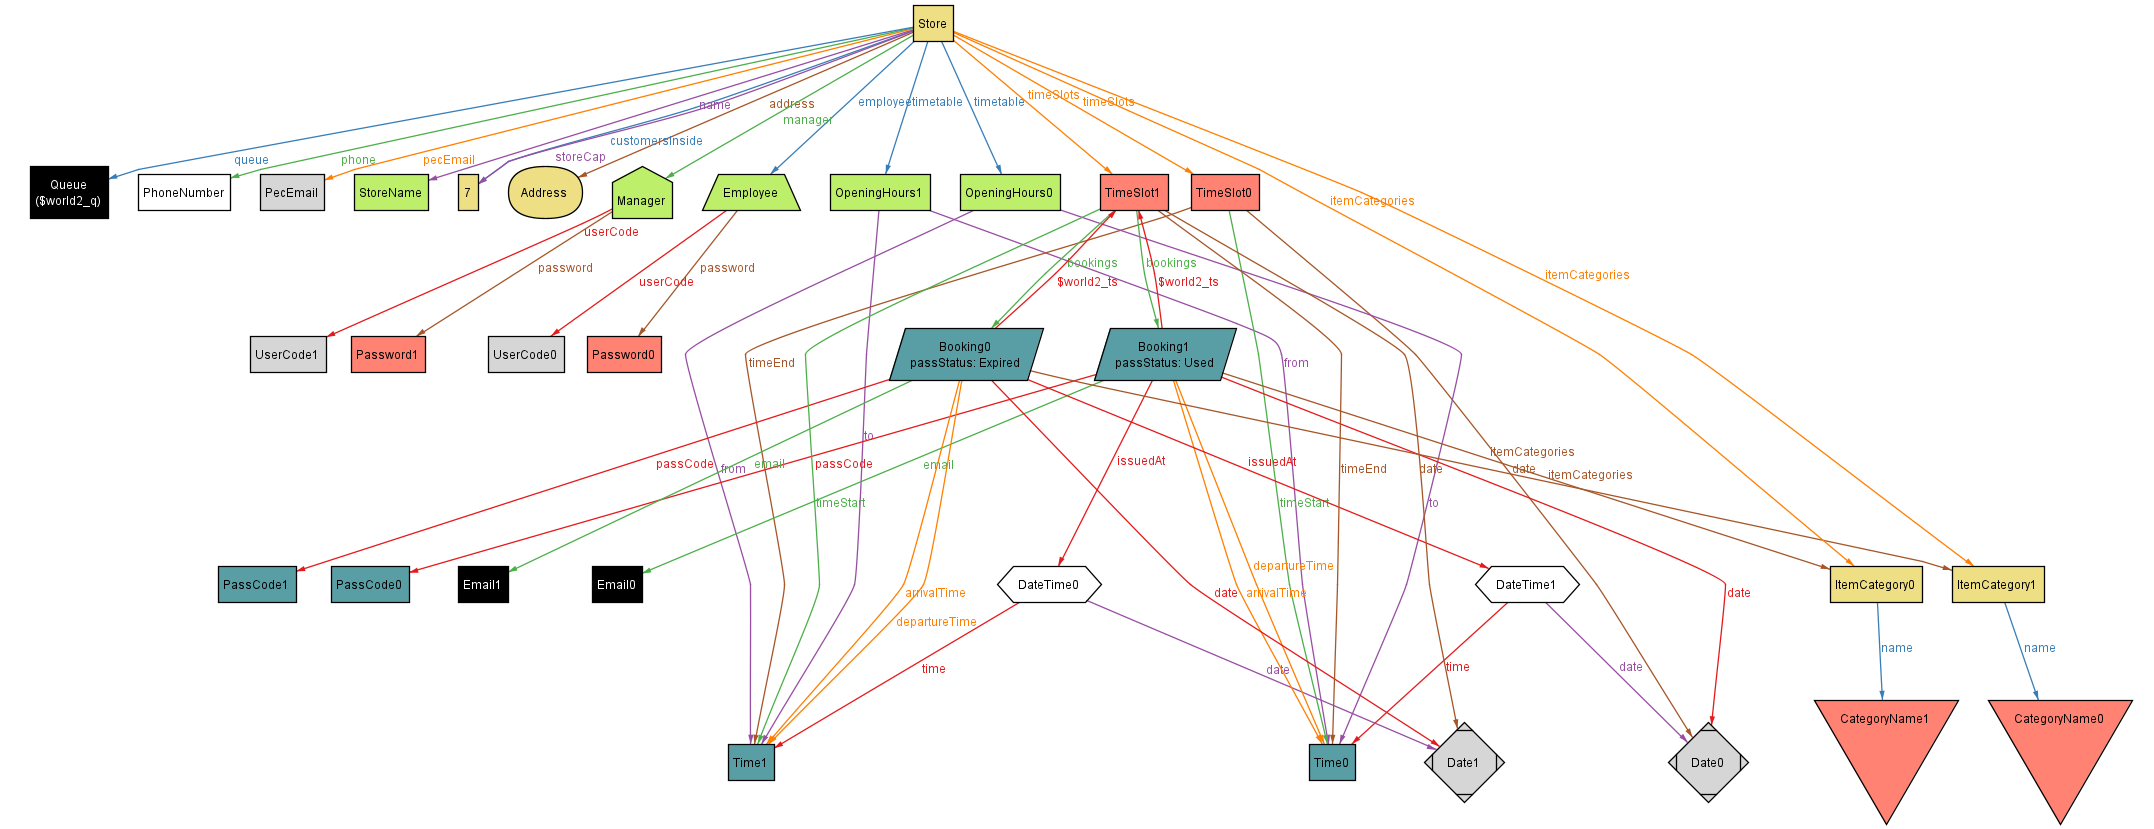
\includegraphics[angle=90,origin=c,height=\textwidth]{world2}
	\caption{Second World.}
	\label{fig:world2}
\end{figure}
\begin{figure}[H]
	\centering
	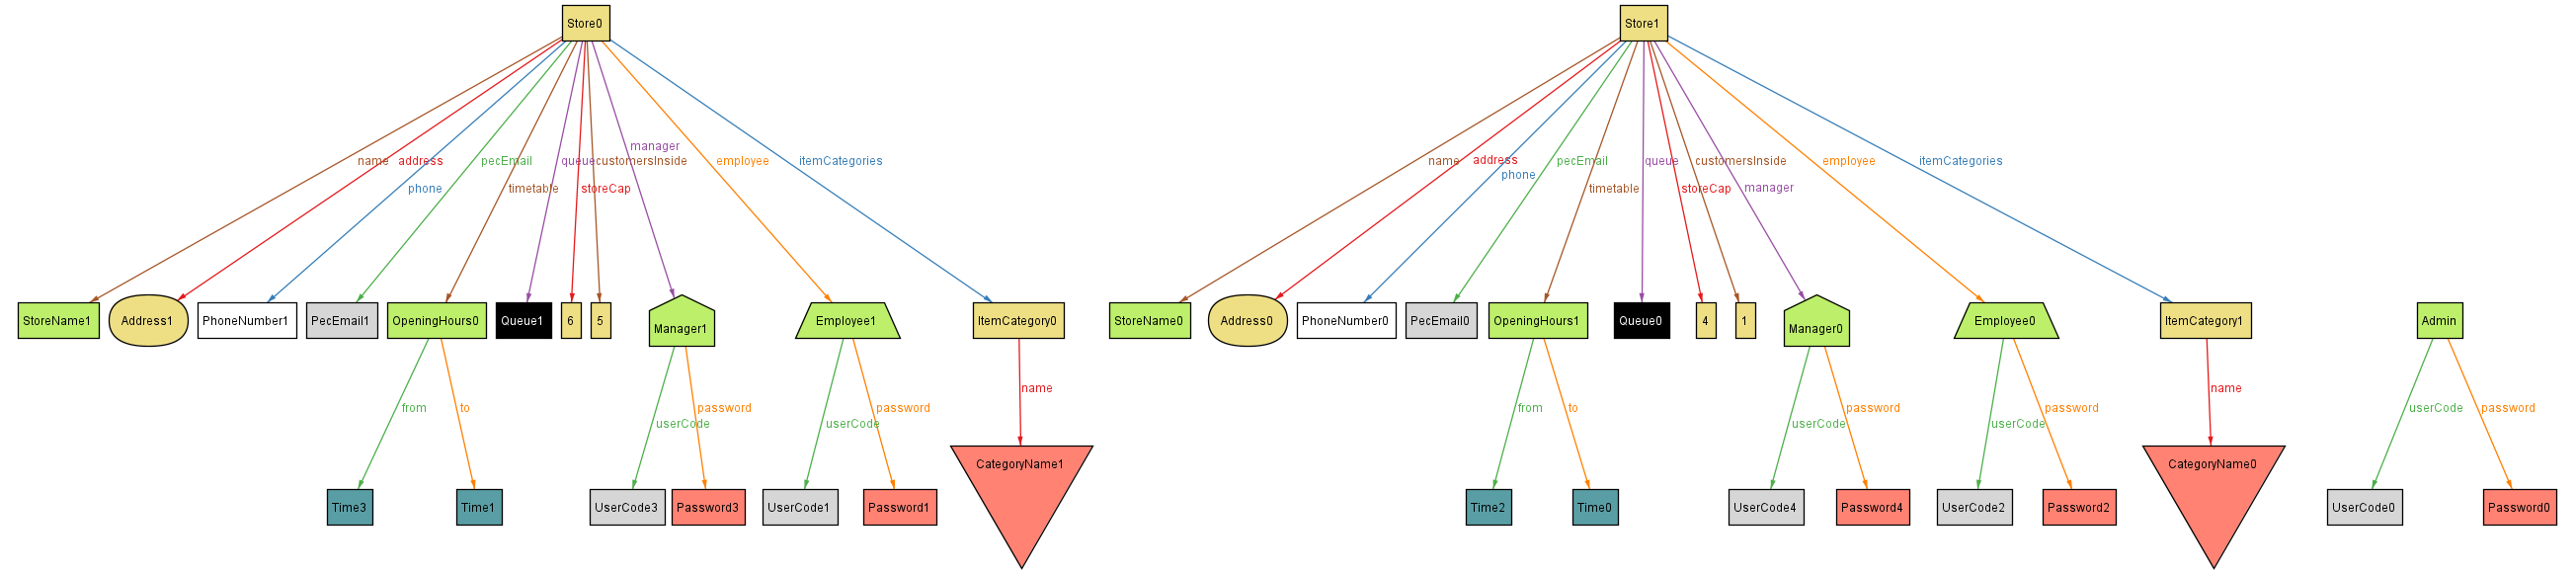
\includegraphics[angle=90,origin=c,height=\textwidth]{world3}
	\caption{Third World.}
	\label{fig:world3}
\end{figure}